\documentclass[11pt,a4paper]{article}

\usepackage[utf8]{inputenc}
\usepackage[ukrainian,english]{babel}
\usepackage{listings}
\usepackage{url}
\usepackage{amsmath,amsthm}
\usepackage{amsfonts}
\usepackage{amssymb}
\usepackage{authblk}
\usepackage{float}
\usepackage{graphicx}

\selectlanguage{english}

\begin{document}

\title{Predicting the translations of red links}
\date{}

\author[ ]{Olga Chernytska}
\author[ ]{Maksym Gontar}
\author[ ]{Kateryna Liubonko}
\author[ ]{Oleksandr Zaytsev}

\affil[ ]{Ukrainian Catholic University}
\affil[ ]{Faculty of Applied Sciences}
\affil[ ]{Lviv, Ukraine}
\affil[ ]{\texttt{\{chernytska,hontar,aloshkina,oleks\}@ucu.edu.ua}}

\maketitle

\begin{abstract}
In this work we propose a technique for matching the red links of Wikipedia to the corresponding articles in another language. We build the graph of all Wikipedia pages and use it to measure similarity between the pages in different languages, one of which exists only as a red link. Such mathing would make the process of filling the gaps in Wikipedia more effective by allowing contributors to translate the existing page that corresponds to a red link rather than writing whole text from scratch.
\end{abstract}

\section{Introduction}

Wikipedia allows its users to create links to the pages that were not yet created. Such links become red and if you click on them, you get redirrected to an empty page and asked to write the missing article. Red links are an important source of information as they let us know what are the gaps in Wikipedia and how important it is to fill them. Every red link is the reference to a non-existing page and the number of such references can serve as a measure of interest that community of contributors has in a certain topic. Filling those gaps is a perfect way of making Wikipedia more complete and interconnected.

A major problem with red links is that because of the way they are stored in database they can not be linked to pages in other languages in a same way as existing pages are linked to their translations. This complicates the contribution process as it is much easier for people to translate and edit the existing page than to write a new one.

We propose a solution for finding the potential translation of the missing pages in other languages. It would allow Wikipedia to automatically match red links to existing pages and make contribution much easier.

\section{Related work}

To our knowledge, there was no work done in this area. In their work The Collaborative Organization of Knowledge, Diomidis Spinellis and Panagiotis Louridas\cite{spinellis} have found that most new articles are created shortly after a corresponding reference to them (red link) is entered into the system and are typically written by different authors from the ones behind the references.

\section{Problem statement}

\begin{enumerate}
	\item Define a distance measure $q: V_{EN} \times V_{UK} \to \mathbb{R}$ that would represent similarity between articles of English ($V_{EN}$) and Ukrainian ($V_{UK}$) Wikipeadia. This measure should be high for articles that are the translations of one another and low for the ones that are not.
	\item For each red link in English Wikipedia find the closest article in Ukrainian Wikipedia in terms of the defined distance measure. In other words, for each $v^{*} \in V_{EN}^{(red)}$ find
	\[ v = \operatorname*{argmin}_{v \in V_{UK}^{(blue)}} q(v^{*}, v) \]
\end{enumerate}

\section{Data collection and preparation}

We have downloaded the full dumps of English\footnote{\url{https://dumps.wikimedia.org/enwiki/20180620/}} and Ukrainian Wikipedia\footnote{\url{https://dumps.wikimedia.org/ukwiki/20180620/}} articles from 20/06/2018. 

Then we have parsed those articles with regular expressions to get outgoing red and blue links: the link article, text and position in the current article text. There was red links in English Wikipedia and red links Ukrainian Wikipedia. There was blue links in English Wikipedia and blue links Ukrainian Wikipedia. This data is stored in enwiki-20180620-pages-links.csv and ukwiki-20180620-pages-links.csv files. Format of those files is following:\\
id - id of a page\\
link\_id - id of a linked page\\
link\_pos - position of link in a page markup text\\  
link\_pos\_perc - relative position of link in a page markup text, range from 0 (at the beginning of page text) to 1 (at the end of page text)\\  
link\_val - title of a linked page\\  
link\_text - link text, if available\\  
is\_red\_link - boolean, whether a link is red or not\\  

Then we have downloaded Wiki interlanguage link records \footnote{\url{https://dumps.wikimedia.org/ukwiki/20180620/ukwiki-20180620-langlinks.sql.gz}} and parsed out all interlingual links between En and Uk Wiki articles. There was 441928 pairs of Uk-En Wiki articles. This data is stored in 20180620-langlinks\_uk\_en.csv file. Format of this file is following:\\
id\_uk - id of a page in Uk Wiki\\
id\_en - id of a linked page in En Wiki\\

From dumps we collected data about pages aliases (redirects) in En and Uk Wiki. The alias page is the page user can come upon by searching the article not by it's original name, but by it's alias name, then user is redirected to the original page. Alias data is important for our task, since links may lead not to the original article, but to it's redirect page. This data is stored in set of files:\\
\\
enwiki-20180620-id\_alias\_title\_alias.csv, ukwiki-20180620-id\_alias\_title\_alias.csv with format:\\
id\_alias - id of alias page\\
title\_alias - title of alias page\\
\\
enwiki-20180620-id\_alias\_id\_orig.csv, ukwiki-20180620-id\_alias\_id\_orig.csv with format:\\
id\_alias - id of alias article\\
id\_orig - id of original article\\
\\
enwiki-20180620-id\_orig\_title\_alias.csv, ukwiki-20180620-id\_orig\_title\_alias.csv with format:\\
id\_orig - id of original article\\
title\_alias - title of alias pages\\

Also we composed a list of all pages in En and Uk Wiki. There were 5669865 in En and 581098 articles Uk Wiki. This data is stored in enwiki-20180620-id\_name.csv, ukwiki-20180620-id\_name.csv files. Format of those files is following:\\ 
id - id of a page\\
title - title of a page\\
length - length of a page markup text\\

Besides that, we did a statistical analysis for red links, we calculated how many times each red link was used and saved results in the enwiki-20180620-red\_name\_count.csv, ukwiki-20180620-red\_name\_count.csv files with format:\\
link\_title - title of a red link\\
in\_count - number of times it was used\\
\\
Also we calculated how many red links there are with a certain number of use, and stored results into the enwiki-20180620-red\_count\_by\_count.csv, ukwiki-20180620-red\_count\_by\_count.csv files with format:\\
count - number of red link usage\\
in\_count - number of this count case\\

For example, in En Wiki red link was used only once for 4354094, and twice for 811612 times.\\

For every eng red link in the matrix we calculate similarity (using similarity metrics selected on the previous step) to those ukr articles that do not have eng version. The most similar ukr article is the one that correeponds to this red link. Possibly, we will find several ukr articles with the same similarities, so add them as candidates for further preprocessing.

\section{Proposed solution}

Among all non-existing articles of English Wikipedia we consider only those that have at least 5 red links pointing to them from existing articles that have translations in Ukrainian Wikipedia. There are 3,593 red articles that satisfy this condition. We look for potential translations of the collected red links in the subset of 82,122 Ukrainian articles that don't have an English translation.

\subsection{Number of common neighbours}

This approach is based on two assumptions:

\begin{enumerate}
	\item Translations of a same article exist in a similar context. Many articles that are connected to them by incoming or outgoing links are also translations of one another.
	\item Let articles $a$ and $b$ be completely unrelated. Let $N(a, b)$ be the total number of links that connect $a$ and $b$ and let $m > n$. Then the probability of $N(a, b) = m$ is lower than the probability of $N(a, b) = n$.
	\item As a result of previous assumption: the greater is the number of links that connect $a$ and $b$ - the higher is the probability that $a$ and $b$ are related.
\end{enumerate}

If article $b$ is references both $a$ and $c$ then assume that $a$ and $c$ are connected by $b$ and the probability of such connection is a joint probability $P(bRa)P(bRc)$ where $R$ is a non-commutative relation "references". And if two articles are a translation of one another, then we think of them as one article.

For eavery given red link $v^{*}$ of English Wikipedia we find the set of articles that reference it.

\[ V_{EN}^{(incoming)} = \{ v \in V_{EN} | vRv^{*} \} \]

Then we find the set of their Ukrainian translations. Here $Q$ is the commutative relation "translation"

\[ V_{UK}^{(transl)} = \{ v \in V_{UK} | \exists w \in V_{EN}^{(incoming)} : vQw \} \]

Next we need a set of all articles of Ukrainian Wikipedia referenced by those translations

\[ V_{UK}^{(outgoing)} = \{ v \in V_{UK} | \exists w in V_{UK}^{(transl)} : wRv \} \]

We define $M: V_{UK}^{(outgoing)} \to \mathbb{N}$ as the number of incoming links from $V_{UK}^{(transl)}$. Now nearest neighbour can be defined as

\[ v = \operatorname*{argmax}_{v \in V_{UK}^{(outgoing)}} M(v) \]

And based on our assumptions, $v$ has the highest probability of satisfying the relation $vQv^{*}$.

%An example of this procedure in given in figure \ref{fig:graph}.

\begin{figure}[H]
  \label{fig:graph}
  \begin{center}
  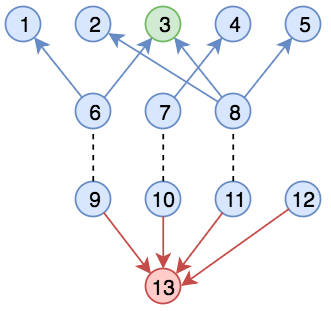
\includegraphics[width=0.36\linewidth]{img/graph}
  \caption{Matching red link with the existing page in other language based on the number of common neighbours. 1-8 are articles of Ukrainian Wikipedia, 9-13 are articles of English Wikipedia. Arrows show links from source to target article (6 references 1), dashed lines connect articles that are translations of each other (6 and 9 are the same article in two languages). We choose 3 as the most likely translation of the red link 13, because it has the most incoming links from the articles whose translations are referencing red article 13. In other words, 3 and 13 have the most neighbours in common. Even though article 12 references 13, it doesn't have Ukrainian translation and therefore it is removed from calculations}
  \end{center}
\end{figure}

We encoded all Ukrainian articles that don't have English translations as bag of words by the unique incoming Ukrainian links. We then encoded every red link as bag of words by its unique incoming English link. Then we mapped such encoding to Ukrainian: every English article in the bag of words was replaced with its corresponding Ukrainian article if it exists, or just removed if not. As a result, both Ukrainian non-translated articles and en red links were encoded in the same feature space - by incoming Ukrainian articles. For every red link we found its Jaccard similarities with all non-translated Ukrainian articles, We reported 5 most similar Ukrainian articles with corresponding Jaccard score for every red link.

\[ J(A, B) = \frac{|A \cap B|}{|A \cup B|} \]

For each red link we reported 5 most likely candidates for its translation\footnote{Source code: \url{https://github.com/olekscode/Power2TheWiki}}.

\subsection{Graph embeddings}

We also tried to encode red links and potential articles in uk wiki with graph embedding techniques. The theoretical and software background for our experiments was based on the paper of Palash Goyal and Emilio Ferrara 'Graph Embedding Techniques, Applications, and Performance: A Survey'\cite{goyal} and their library GEM\footnote{\url{https://github.com/palash1992/GEM}}.

Among different embedding techniques described in that article and implemented in the library we have chosen Locally Linear Embedding and Structural Deep Network Embedding (SDNE). The choice of Locally Linear Embedding was due to way it embedded the nodes - it assumes that every node is a linear combination of its neighbors in the embedding space. It suited to our task as the information of the articles with their outcoming links (including red links) for now is the only information which could help to distinguish between different articles. SDNE was chosen due to its good results in experiments provided by authors of the article.

For embedding we assumed that the information we need is all links between articles in Ukrainian wikipedia and the articles from English wikipedia for which we are looking the correspondences in Uk wiki. So we excluded all other information about links in English wiki as it would add noise in our dataset and make it much larger. Nevertheless this data was too huge for the library and our hardware so we kept information only on red articles their 'parent' articles with ids in Ukrainian wiki and all the outcoming links of these 'parent' articles in Uk wiki among which could be potential equivalences for red articles.
Totally the graph which we embedded has size 99629 nodes and 348948 edges.
Locally Linear Embedding technique didn't work for us and it need further investigation of the cause of fail but SDNE gave us the first embedding of our graph.

\section{Evaluation}

We evaluated algorithm performance manually, as it is impossible to find threshold for Jaccard similarity, and correct corresponding Ukrainian article is not always the first among the 5 most similar articles. For about a third among 3,593 red link, algorithm didn't found any similar articles. However, for 165 en red links true corresponding non-translated Ukrainian article were found.

\begin{table}[H]
\caption{Some examples of matched articles}

\begin{center}
\begin{tabular}{|l|l|}
\hline
\textbf{Red English article} & \textbf{Matched Ukrainian article} \\
\hline
Roksana Zasina & \foreignlanguage{ukrainian}{Роксана Засіна} \\
3rd Ukrainian Verkhovna Rada & \foreignlanguage{ukrainian}{Верховна Рада України III скликання} \\
Oleksandr Derdo & \foreignlanguage{ukrainian}{Дердо Олександр Вікторович} \\
2003 European Wrestling Championships & \foreignlanguage{ukrainian}{Чемпіонат Європи з боротьби 2003} \\
Marcus Atilius Regulus Calenus & \foreignlanguage{ukrainian}{Марк Атілій Регул Кален} \\
\hline
\end{tabular}
\end{center}
\end{table}

\section{Conclusions}

We provided a list of en red articles for which we found corresponding uk non-translated articles. Such articles are about people, films and places in Ukraine, mostly connected with sport, and about Roman Emperors (with no obvious reasons). We sorted these red links based on number of incoming links from en wiki. We assume that those red links, that have more incoming en links, are more valuable for wikipedia community, and their corresponding uk articles are best candidates for translation.

\bibliographystyle{plain}
\bibliography{Power2TheWiki}

\end{document}